\section{\sysbench: A Benchmark for Agent-Task Efficiency}
\label{sec:benchmark}




Evaluating the agent-task efficiency of a training framework requires
varying the framework while holding the agent and task fixed. This is
the inverse of standard benchmarks for AI coding agents~\cite{jimenez2024swebench,chen2021evaluatinglargelanguagemodels,austin2021programsynthesislargelanguage},
which hold the codebase and task fixed and vary the agent to score
capability. We introduce \sysbench,
a benchmark with a fixed agent and curated task suite run across
frameworks, so that differences in agent performance are
attributable to framework design. The suite spans the kinds of work
researchers typically perform on training frameworks, organized
around three recurring patterns: understanding the framework
without modifying it, operating it as a tool for instrumentation
and profiling, and extending it with new functionality. Tasks are distributed across three categories:
\squishlist
  \vspace{-3pt}
  \item Q\&A (12 tasks): answer questions whose answer is a
  property of the code, not a runtime measurement (e.g., ``how is
  the device mesh built?'').
  \vspace{-3pt}
  \item Operate and Profile (4 tasks): run, instrument, and
  profile the framework as a tool (e.g., capture an Nsight Systems
  profile and identify the most expensive CUDA kernels).
  \vspace{-3pt}
  \item New Feature (4 tasks): port a new model architecture into
  the framework end-to-end against a published reference
  implementation (e.g., Mixture of Block Attention
  (MoBA)~\cite{lu2025moba}).
  \vspace{-3pt}
\squishend


\autoref{fig:benchmark-harness} illustrates the agent loop for each
category, with agent involvement deepening from Q\&A (read-only)
to Operate and Profile (running, minor instrumentation) to New
Feature (substantial modification, test-driven iteration). Full
task descriptions and per-category correctness checks are in
Appendix~\ref{sec:appendix:tasks}. Using \sysbench, we evaluate
\sys and production frameworks, reporting five effort metrics:
session duration, active GPU time, agent turns, per-turn context,
and output tokens. Without a single-scalar metric for agent-task
efficiency, we report each dimension independently.

Q\&A questions are chosen to be valid across all three
frameworks, excluding framework-specific behaviors.
\sysbench does not cover tasks like cross-model propagation of
a shared change, where production frameworks' implicit
indirection may lower agent effort; we leave these as future work.

\begin{figure}[t]
  \centering
  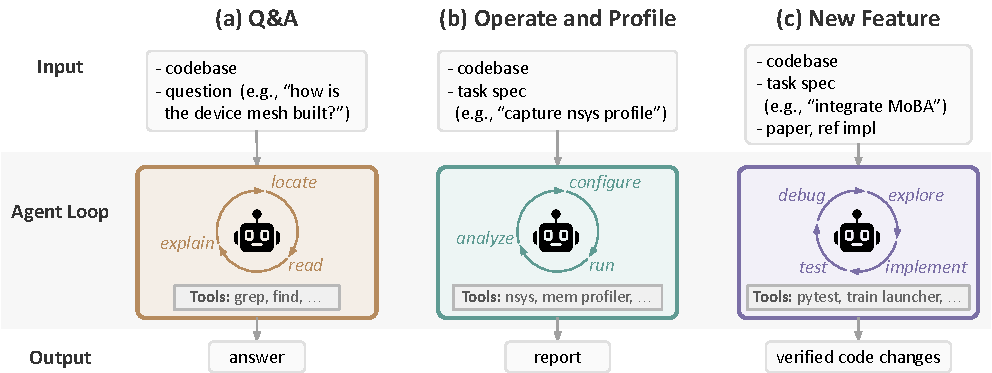
\includegraphics[width=0.85\textwidth]{figures/fig5_agent_loop.pdf}
  \caption{Per-category agent loop. Steps, tools, and output differ across categories.
  }
  \vspace{-9pt}
  \label{fig:benchmark-harness}
\end{figure}
